% Options for packages loaded elsewhere
\PassOptionsToPackage{unicode}{hyperref}
\PassOptionsToPackage{hyphens}{url}
\documentclass[
]{article}
\usepackage{xcolor}
\usepackage[margin=1in]{geometry}
\usepackage{amsmath,amssymb}
\setcounter{secnumdepth}{-\maxdimen} % remove section numbering
\usepackage{iftex}
\ifPDFTeX
  \usepackage[T1]{fontenc}
  \usepackage[utf8]{inputenc}
  \usepackage{textcomp} % provide euro and other symbols
\else % if luatex or xetex
  \usepackage{unicode-math} % this also loads fontspec
  \defaultfontfeatures{Scale=MatchLowercase}
  \defaultfontfeatures[\rmfamily]{Ligatures=TeX,Scale=1}
\fi
\usepackage{lmodern}
\ifPDFTeX\else
  % xetex/luatex font selection
\fi
% Use upquote if available, for straight quotes in verbatim environments
\IfFileExists{upquote.sty}{\usepackage{upquote}}{}
\IfFileExists{microtype.sty}{% use microtype if available
  \usepackage[]{microtype}
  \UseMicrotypeSet[protrusion]{basicmath} % disable protrusion for tt fonts
}{}
\makeatletter
\@ifundefined{KOMAClassName}{% if non-KOMA class
  \IfFileExists{parskip.sty}{%
    \usepackage{parskip}
  }{% else
    \setlength{\parindent}{0pt}
    \setlength{\parskip}{6pt plus 2pt minus 1pt}}
}{% if KOMA class
  \KOMAoptions{parskip=half}}
\makeatother
\usepackage{color}
\usepackage{fancyvrb}
\newcommand{\VerbBar}{|}
\newcommand{\VERB}{\Verb[commandchars=\\\{\}]}
\DefineVerbatimEnvironment{Highlighting}{Verbatim}{commandchars=\\\{\}}
% Add ',fontsize=\small' for more characters per line
\usepackage{framed}
\definecolor{shadecolor}{RGB}{248,248,248}
\newenvironment{Shaded}{\begin{snugshade}}{\end{snugshade}}
\newcommand{\AlertTok}[1]{\textcolor[rgb]{0.94,0.16,0.16}{#1}}
\newcommand{\AnnotationTok}[1]{\textcolor[rgb]{0.56,0.35,0.01}{\textbf{\textit{#1}}}}
\newcommand{\AttributeTok}[1]{\textcolor[rgb]{0.13,0.29,0.53}{#1}}
\newcommand{\BaseNTok}[1]{\textcolor[rgb]{0.00,0.00,0.81}{#1}}
\newcommand{\BuiltInTok}[1]{#1}
\newcommand{\CharTok}[1]{\textcolor[rgb]{0.31,0.60,0.02}{#1}}
\newcommand{\CommentTok}[1]{\textcolor[rgb]{0.56,0.35,0.01}{\textit{#1}}}
\newcommand{\CommentVarTok}[1]{\textcolor[rgb]{0.56,0.35,0.01}{\textbf{\textit{#1}}}}
\newcommand{\ConstantTok}[1]{\textcolor[rgb]{0.56,0.35,0.01}{#1}}
\newcommand{\ControlFlowTok}[1]{\textcolor[rgb]{0.13,0.29,0.53}{\textbf{#1}}}
\newcommand{\DataTypeTok}[1]{\textcolor[rgb]{0.13,0.29,0.53}{#1}}
\newcommand{\DecValTok}[1]{\textcolor[rgb]{0.00,0.00,0.81}{#1}}
\newcommand{\DocumentationTok}[1]{\textcolor[rgb]{0.56,0.35,0.01}{\textbf{\textit{#1}}}}
\newcommand{\ErrorTok}[1]{\textcolor[rgb]{0.64,0.00,0.00}{\textbf{#1}}}
\newcommand{\ExtensionTok}[1]{#1}
\newcommand{\FloatTok}[1]{\textcolor[rgb]{0.00,0.00,0.81}{#1}}
\newcommand{\FunctionTok}[1]{\textcolor[rgb]{0.13,0.29,0.53}{\textbf{#1}}}
\newcommand{\ImportTok}[1]{#1}
\newcommand{\InformationTok}[1]{\textcolor[rgb]{0.56,0.35,0.01}{\textbf{\textit{#1}}}}
\newcommand{\KeywordTok}[1]{\textcolor[rgb]{0.13,0.29,0.53}{\textbf{#1}}}
\newcommand{\NormalTok}[1]{#1}
\newcommand{\OperatorTok}[1]{\textcolor[rgb]{0.81,0.36,0.00}{\textbf{#1}}}
\newcommand{\OtherTok}[1]{\textcolor[rgb]{0.56,0.35,0.01}{#1}}
\newcommand{\PreprocessorTok}[1]{\textcolor[rgb]{0.56,0.35,0.01}{\textit{#1}}}
\newcommand{\RegionMarkerTok}[1]{#1}
\newcommand{\SpecialCharTok}[1]{\textcolor[rgb]{0.81,0.36,0.00}{\textbf{#1}}}
\newcommand{\SpecialStringTok}[1]{\textcolor[rgb]{0.31,0.60,0.02}{#1}}
\newcommand{\StringTok}[1]{\textcolor[rgb]{0.31,0.60,0.02}{#1}}
\newcommand{\VariableTok}[1]{\textcolor[rgb]{0.00,0.00,0.00}{#1}}
\newcommand{\VerbatimStringTok}[1]{\textcolor[rgb]{0.31,0.60,0.02}{#1}}
\newcommand{\WarningTok}[1]{\textcolor[rgb]{0.56,0.35,0.01}{\textbf{\textit{#1}}}}
\usepackage{graphicx}
\makeatletter
\newsavebox\pandoc@box
\newcommand*\pandocbounded[1]{% scales image to fit in text height/width
  \sbox\pandoc@box{#1}%
  \Gscale@div\@tempa{\textheight}{\dimexpr\ht\pandoc@box+\dp\pandoc@box\relax}%
  \Gscale@div\@tempb{\linewidth}{\wd\pandoc@box}%
  \ifdim\@tempb\p@<\@tempa\p@\let\@tempa\@tempb\fi% select the smaller of both
  \ifdim\@tempa\p@<\p@\scalebox{\@tempa}{\usebox\pandoc@box}%
  \else\usebox{\pandoc@box}%
  \fi%
}
% Set default figure placement to htbp
\def\fps@figure{htbp}
\makeatother
\setlength{\emergencystretch}{3em} % prevent overfull lines
\providecommand{\tightlist}{%
  \setlength{\itemsep}{0pt}\setlength{\parskip}{0pt}}
\usepackage{bookmark}
\IfFileExists{xurl.sty}{\usepackage{xurl}}{} % add URL line breaks if available
\urlstyle{same}
\hypersetup{
  pdftitle={Regresní analýza},
  hidelinks,
  pdfcreator={LaTeX via pandoc}}

\title{Regresní analýza}
\author{}
\date{\vspace{-2.5em}}

\begin{document}
\maketitle

\subsection{LMER model - fixní efekty,
K}\label{lmer-model---fixnuxed-efekty-k}

Mnohem lepší \(R^2\), stále malé. Nevýznamný poměr \(S/K\) a styl
využití opce (a model).

\begin{Shaded}
\begin{Highlighting}[]
\NormalTok{subset\_args }\OtherTok{\textless{}{-}} \FunctionTok{c}\NormalTok{(}
  \CommentTok{\#"S",}
  \StringTok{"moneyness"}\NormalTok{,}
  \StringTok{"K"}\NormalTok{,}
  \StringTok{"r"}\NormalTok{,}
  \StringTok{"sigma"}\NormalTok{,}
  \StringTok{"q"}\NormalTok{,}
  \StringTok{"T"}\NormalTok{,}
  \StringTok{"am\_eu"}\NormalTok{,}
  \StringTok{"call\_put"}\NormalTok{,}
  \StringTok{"model"}\NormalTok{,}
  \StringTok{"ticker"}\NormalTok{,}
  \StringTok{"snapshot\_month"}
\NormalTok{)}
\NormalTok{interactions }\OtherTok{\textless{}{-}} \FunctionTok{c}\NormalTok{()}

\NormalTok{rhs }\OtherTok{\textless{}{-}} \FunctionTok{paste}\NormalTok{(}\FunctionTok{c}\NormalTok{(subset\_args, interactions), }\AttributeTok{collapse =} \StringTok{" + "}\NormalTok{)}
\NormalTok{formula }\OtherTok{\textless{}{-}} \FunctionTok{as.formula}\NormalTok{(}\FunctionTok{paste}\NormalTok{(}\StringTok{"pricing\_error \textasciitilde{} "}\NormalTok{, rhs))}

\NormalTok{rmr\_relative }\OtherTok{\textless{}{-}} \FunctionTok{lm}\NormalTok{(formula, }\AttributeTok{data =}\NormalTok{ train\_data\_rel)}
\end{Highlighting}
\end{Shaded}

\begin{Shaded}
\begin{Highlighting}[]
\FunctionTok{summary}\NormalTok{(rmr\_relative)}
\end{Highlighting}
\end{Shaded}

\begin{verbatim}
## 
## Call:
## lm(formula = formula, data = train_data_rel)
## 
## Residuals:
##       Min        1Q    Median        3Q       Max 
## -0.116244 -0.005499  0.001000  0.007341  0.085975 
## 
## Coefficients: (1 not defined because of singularities)
##                    Estimate Std. Error t value Pr(>|t|)    
## (Intercept)      -2.943e-02  1.279e-03 -23.013  < 2e-16 ***
## moneyness         9.768e-05  3.310e-05   2.951 0.003168 ** 
## K                -6.876e-06  1.599e-07 -42.999  < 2e-16 ***
## r                 1.776e+00  2.854e-02  62.203  < 2e-16 ***
## sigma            -7.635e-02  1.244e-03 -61.358  < 2e-16 ***
## q                -5.167e-01  4.951e-02 -10.436  < 2e-16 ***
## T                 3.834e-03  4.181e-05  91.718  < 2e-16 ***
## am_eueuropean    -2.130e-03  5.683e-04  -3.748 0.000178 ***
## call_putputs     -3.068e-03  6.041e-05 -50.779  < 2e-16 ***
## modeluser_crr    -1.476e-05  7.081e-05  -0.208 0.834903    
## modeluser_mc     -5.503e-05  7.085e-05  -0.777 0.437304    
## ticker^XDA       -4.432e-02  1.929e-03 -22.980  < 2e-16 ***
## ticker^XDB       -1.256e-02  1.625e-03  -7.731 1.07e-14 ***
## ticker^XDE       -2.507e-02  1.180e-03 -21.248  < 2e-16 ***
## ticker^XDN       -1.685e-02  1.431e-03 -11.776  < 2e-16 ***
## tickerAAPL       -1.387e-02  4.239e-04 -32.719  < 2e-16 ***
## tickerAMD         8.940e-03  1.571e-04  56.899  < 2e-16 ***
## tickerAMZN       -5.636e-03  3.181e-04 -17.719  < 2e-16 ***
## tickerGOOGL       1.245e-03  4.079e-04   3.053 0.002266 ** 
## tickerJNJ         1.671e-03  1.738e-03   0.961 0.336381    
## tickerKO         -4.758e-03  1.587e-03  -2.998 0.002719 ** 
## tickerMETA       -4.490e-03  3.017e-04 -14.880  < 2e-16 ***
## tickerMSFT       -5.288e-03  5.642e-04  -9.372  < 2e-16 ***
## tickerNFLX       -4.631e-03  3.123e-04 -14.831  < 2e-16 ***
## tickerNVDA        1.677e-03  2.265e-04   7.404 1.32e-13 ***
## tickerPG         -3.174e-03  1.439e-03  -2.205 0.027431 *  
## tickerTSLA               NA         NA      NA       NA    
## snapshot_month02  1.472e-03  8.430e-05  17.465  < 2e-16 ***
## snapshot_month03 -2.282e-05  8.941e-05  -0.255 0.798513    
## snapshot_month05  1.251e-03  1.091e-04  11.460  < 2e-16 ***
## ---
## Signif. codes:  0 '***' 0.001 '**' 0.01 '*' 0.05 '.' 0.1 ' ' 1
## 
## Residual standard error: 0.0166 on 329483 degrees of freedom
## Multiple R-squared:  0.1728, Adjusted R-squared:  0.1728 
## F-statistic:  2459 on 28 and 329483 DF,  p-value: < 2.2e-16
\end{verbatim}

\begin{Shaded}
\begin{Highlighting}[]
\FunctionTok{r2}\NormalTok{(rmr\_relative)}
\end{Highlighting}
\end{Shaded}

\begin{verbatim}
## # R2 for Linear Regression
##        R2: 0.173
##   adj. R2: 0.173
\end{verbatim}

\begin{verbatim}
## Model matrix is rank deficient. Parameters `tickerTSLA` were not
##   estimable.
\end{verbatim}

\pandocbounded{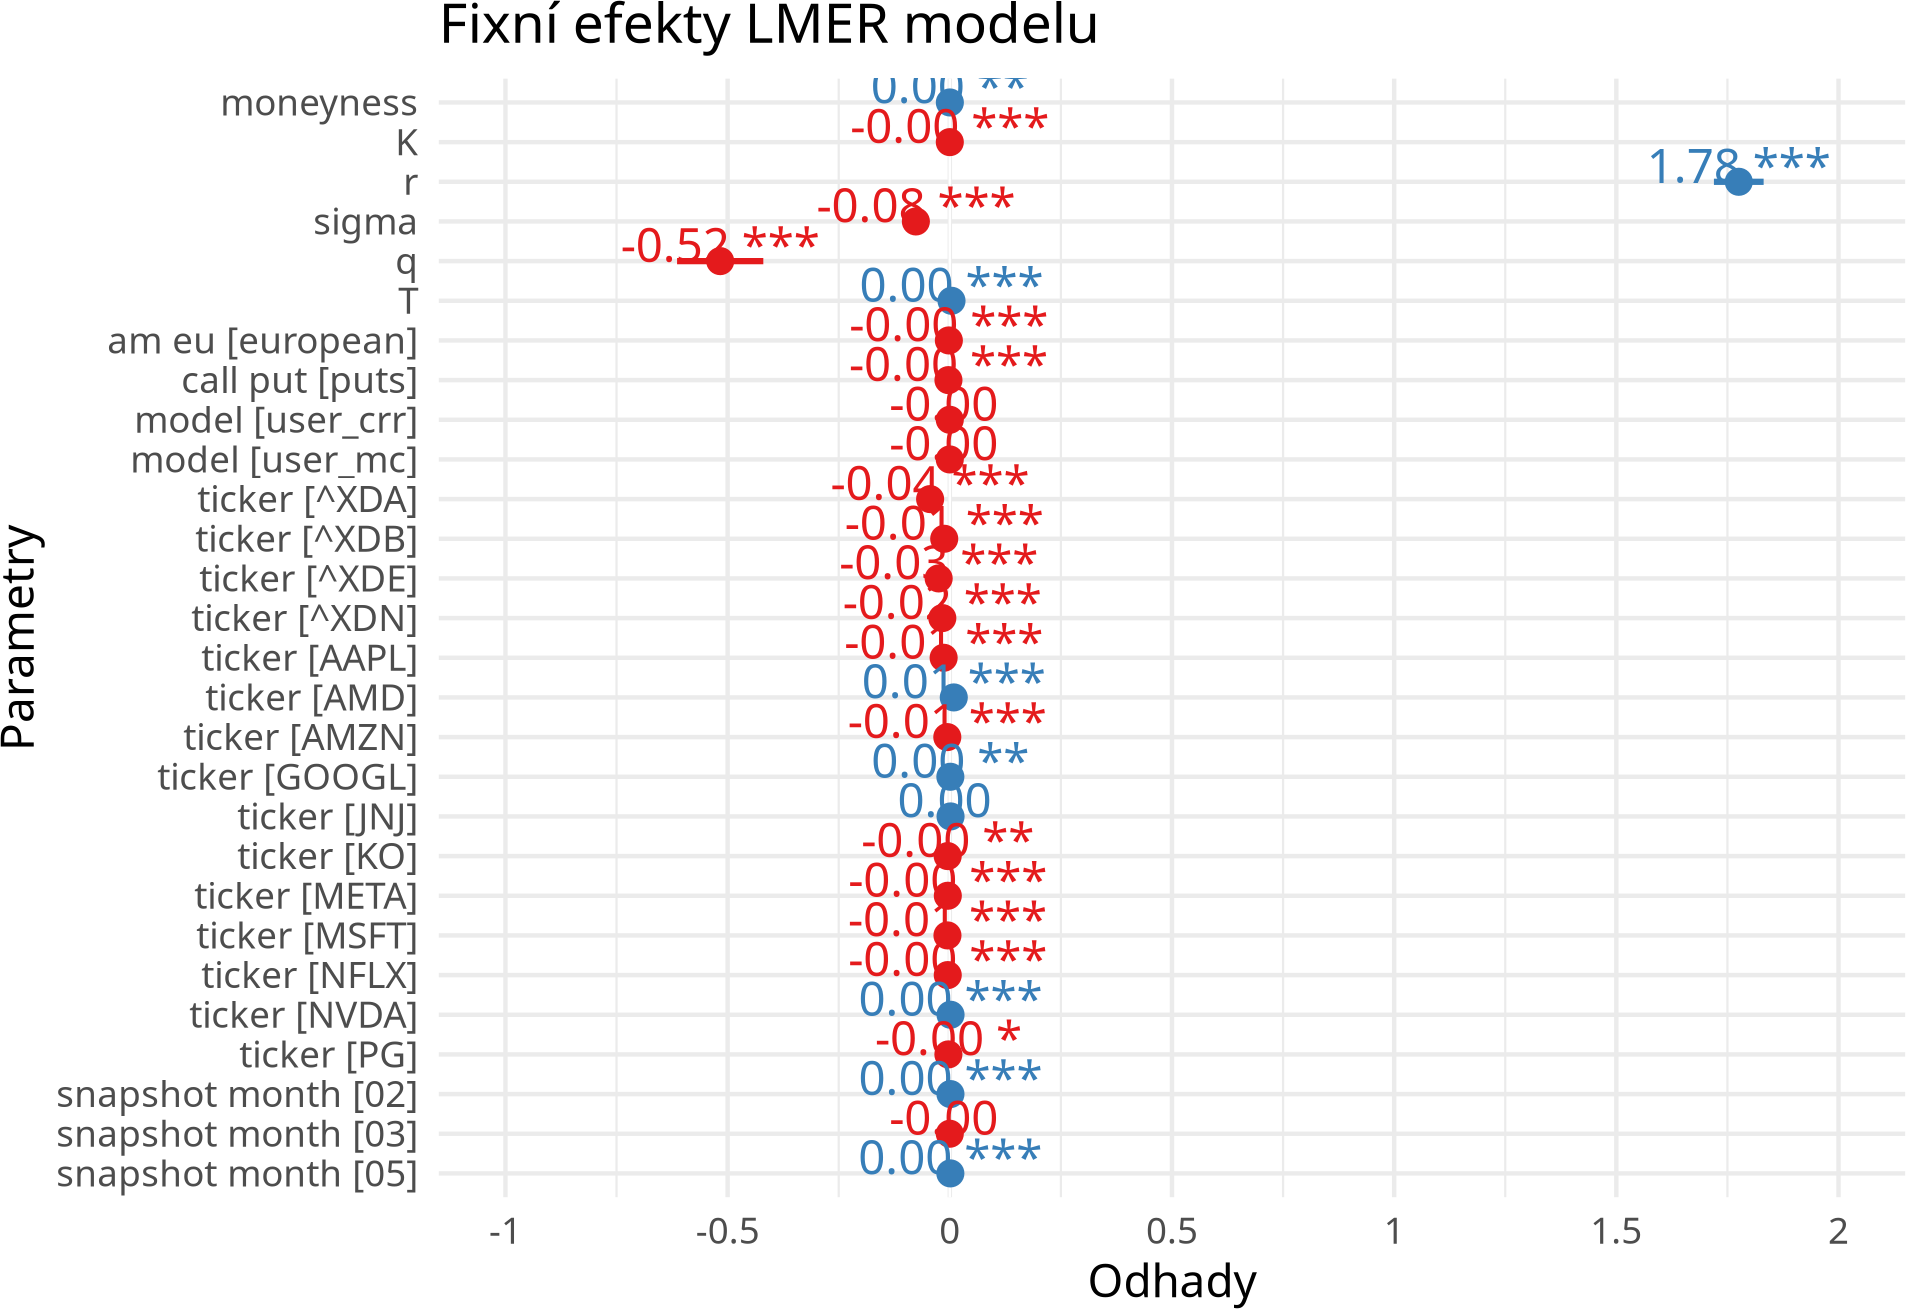
\includegraphics[keepaspectratio]{regression3_files/regression3_files/figure-latex/unnamed-chunk-3-1.png}}

\pandocbounded{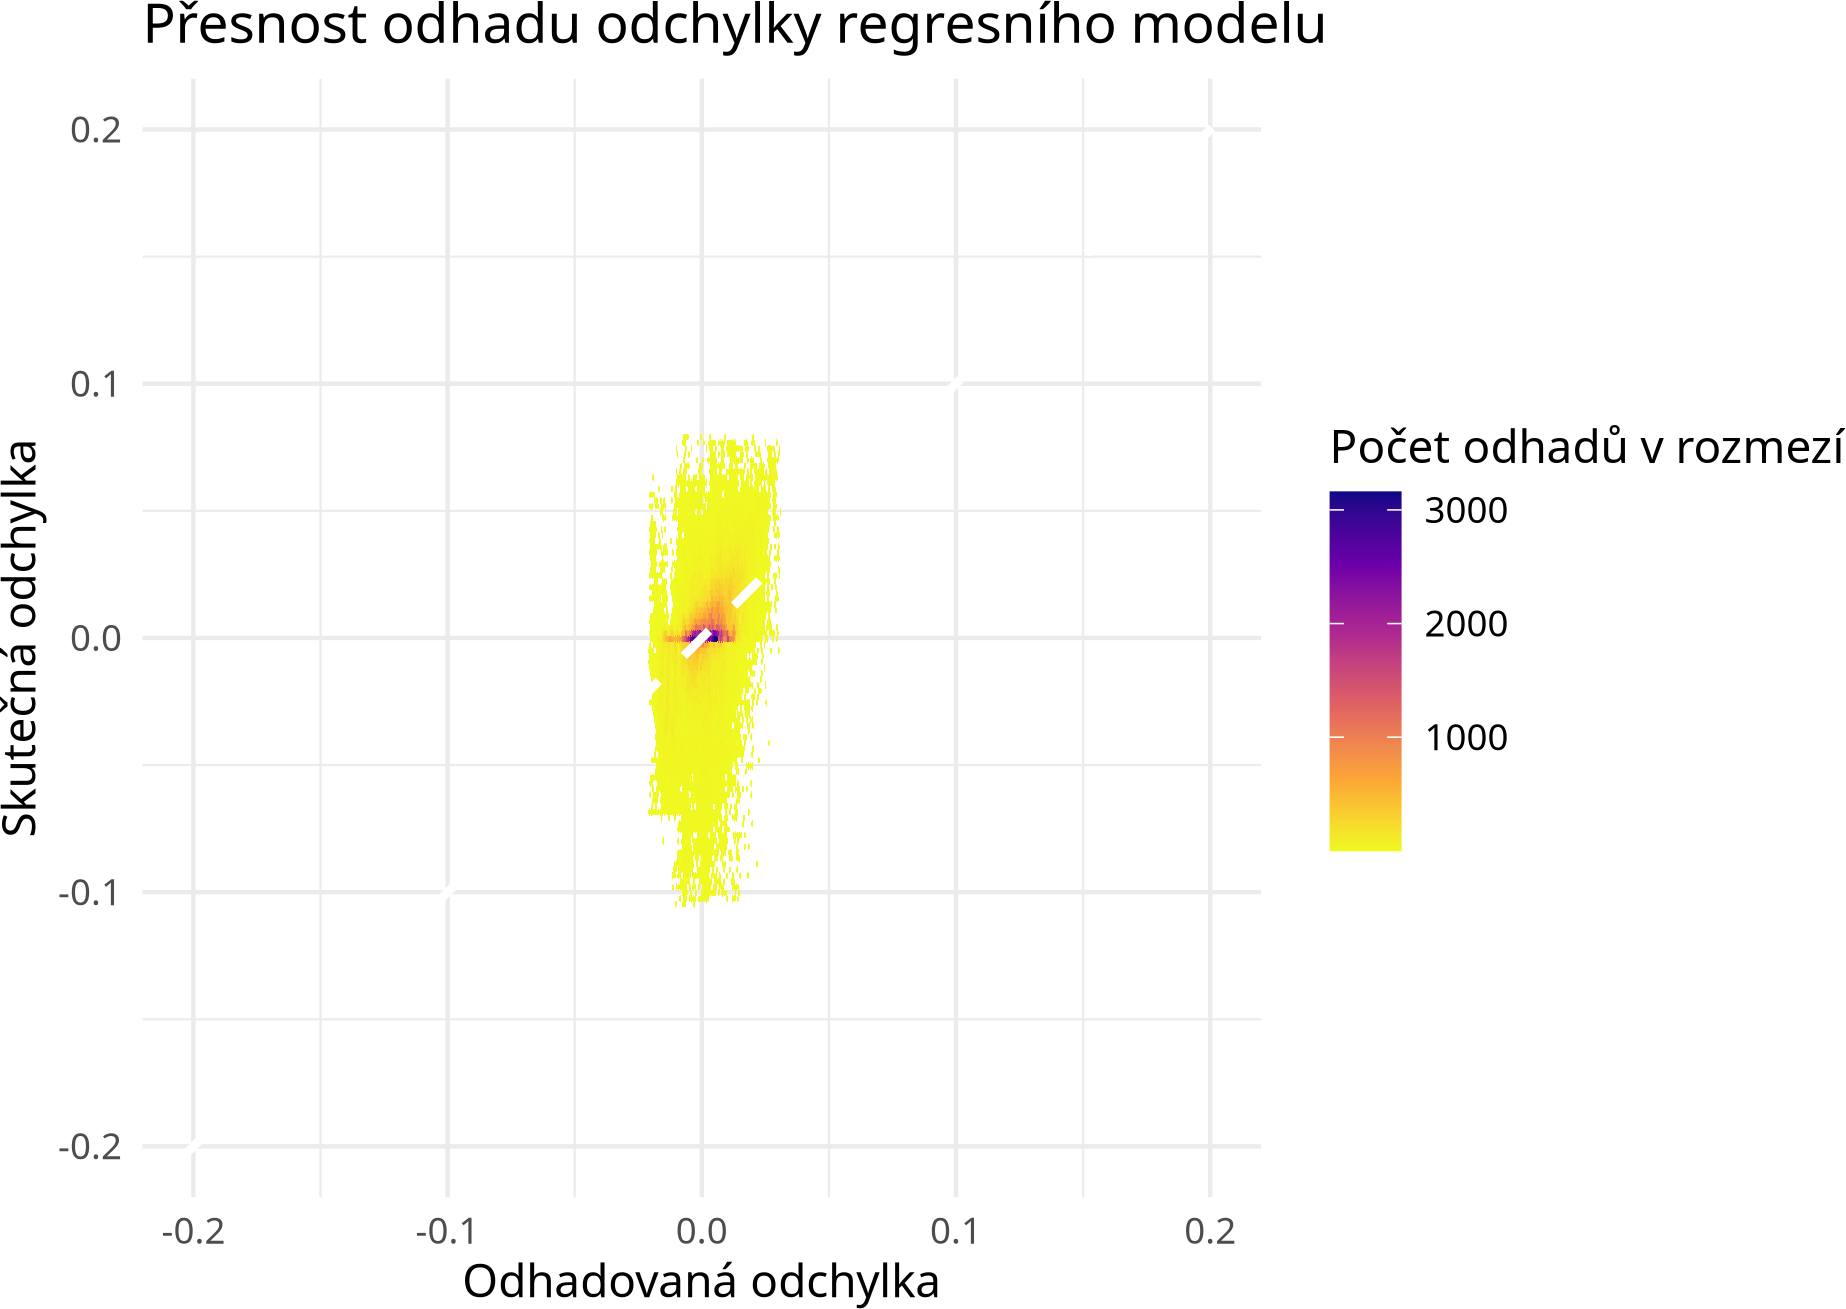
\includegraphics[keepaspectratio]{regression3_files/regression3_files/figure-latex/prediction_fixed_K-1.png}}

\begin{Shaded}
\begin{Highlighting}[]
\FunctionTok{anova}\NormalTok{(rmr\_relative)}
\end{Highlighting}
\end{Shaded}

\begin{verbatim}
## Analysis of Variance Table
## 
## Response: pricing_error
##                    Df Sum Sq Mean Sq    F value Pr(>F)    
## moneyness           1  0.124  0.1242   450.5876 <2e-16 ***
## K                   1  0.690  0.6898  2503.0910 <2e-16 ***
## r                   1  1.935  1.9346  7020.1455 <2e-16 ***
## sigma               1  6.870  6.8704 24930.8467 <2e-16 ***
## q                   1  1.141  1.1413  4141.6189 <2e-16 ***
## T                   1  2.256  2.2561  8186.8529 <2e-16 ***
## am_eu               1  0.110  0.1102   400.0206 <2e-16 ***
## call_put            1  0.772  0.7721  2801.6368 <2e-16 ***
## model               2  0.000  0.0001     0.2836  0.753    
## ticker             15  4.938  0.3292  1194.5631 <2e-16 ***
## snapshot_month      3  0.136  0.0453   164.5608 <2e-16 ***
## Residuals      329483 90.798  0.0003                      
## ---
## Signif. codes:  0 '***' 0.001 '**' 0.01 '*' 0.05 '.' 0.1 ' ' 1
\end{verbatim}

\begin{Shaded}
\begin{Highlighting}[]
\FunctionTok{ranef}\NormalTok{(rmr\_relative)}
\end{Highlighting}
\end{Shaded}

\subsection{LMER model - náhodné efekty,
K}\label{lmer-model---nuxe1hodnuxe9-efekty-k}

Mnohem lepší \(R^2\), stále malé. Nevýznamný poměr \(S/K\) a styl
využití opce (a model).

\begin{Shaded}
\begin{Highlighting}[]
\NormalTok{subset\_args }\OtherTok{\textless{}{-}} \FunctionTok{c}\NormalTok{(}
  \CommentTok{\#"S",}
  \StringTok{"moneyness"}\NormalTok{,}
  \StringTok{"K"}\NormalTok{,}
  \StringTok{"r"}\NormalTok{,}
  \StringTok{"sigma"}\NormalTok{,}
  \StringTok{"q"}\NormalTok{,}
  \StringTok{"T"}\NormalTok{,}
  \StringTok{"am\_eu"}\NormalTok{,}
  \StringTok{"call\_put"}\NormalTok{,}
  \StringTok{"model"}
  \CommentTok{\#"ticker"}
\NormalTok{)}
\NormalTok{interactions }\OtherTok{\textless{}{-}} \FunctionTok{c}\NormalTok{(}
  \StringTok{"(1 | ticker)"}\NormalTok{,}
  \StringTok{"(1 | snapshot\_month)"}
\NormalTok{)}

\NormalTok{rhs }\OtherTok{\textless{}{-}} \FunctionTok{paste}\NormalTok{(}\FunctionTok{c}\NormalTok{(subset\_args, interactions), }\AttributeTok{collapse =} \StringTok{" + "}\NormalTok{)}
\NormalTok{formula }\OtherTok{\textless{}{-}} \FunctionTok{as.formula}\NormalTok{(}\FunctionTok{paste}\NormalTok{(}\StringTok{"pricing\_error \textasciitilde{} "}\NormalTok{, rhs))}

\NormalTok{rmr\_relative }\OtherTok{\textless{}{-}} \FunctionTok{lmer}\NormalTok{(formula, }\AttributeTok{data =}\NormalTok{ train\_data\_rel)}
\end{Highlighting}
\end{Shaded}

\begin{verbatim}
## Warning: Some predictor variables are on very different scales: consider rescaling. 
## You may also use (g)lmerControl(autoscale = TRUE) to improve numerical stability.
## Warning: Some predictor variables are on very different scales: consider rescaling. 
## You may also use (g)lmerControl(autoscale = TRUE) to improve numerical stability.
\end{verbatim}

\begin{Shaded}
\begin{Highlighting}[]
\FunctionTok{summary}\NormalTok{(rmr\_relative)}
\end{Highlighting}
\end{Shaded}

\begin{verbatim}
## Linear mixed model fit by REML. t-tests use Satterthwaite's method [
## lmerModLmerTest]
## Formula: formula
##    Data: train_data_rel
## 
## REML criterion at convergence: -1765482
## 
## Scaled residuals: 
##     Min      1Q  Median      3Q     Max 
## -7.0018 -0.3312  0.0603  0.4421  5.1790 
## 
## Random effects:
##  Groups         Name        Variance  Std.Dev. 
##  ticker         (Intercept) 9.274e-05 0.0096303
##  snapshot_month (Intercept) 6.348e-07 0.0007967
##  Residual                   2.756e-04 0.0166005
## Number of obs: 329512, groups:  ticker, 17; snapshot_month, 4
## 
## Fixed effects:
##                 Estimate Std. Error         df t value Pr(>|t|)    
## (Intercept)   -3.112e-02  3.066e-03  2.132e+01 -10.148 1.28e-09 ***
## moneyness      9.925e-05  3.310e-05  3.284e+05   2.999  0.00271 ** 
## K             -6.861e-06  1.598e-07  3.163e+05 -42.939  < 2e-16 ***
## r              1.775e+00  2.850e-02  1.758e+05  62.275  < 2e-16 ***
## sigma         -7.630e-02  1.240e-03  1.024e+05 -61.544  < 2e-16 ***
## q             -5.176e-01  4.834e-02  6.502e+03 -10.709  < 2e-16 ***
## T              3.834e-03  4.181e-05  3.294e+05  91.704  < 2e-16 ***
## am_eueuropean -1.939e-02  5.190e-03  1.520e+01  -3.735  0.00195 ** 
## call_putputs  -3.066e-03  6.041e-05  3.295e+05 -50.752  < 2e-16 ***
## modeluser_crr -1.471e-05  7.081e-05  3.295e+05  -0.208  0.83538    
## modeluser_mc  -5.500e-05  7.085e-05  3.295e+05  -0.776  0.43757    
## ---
## Signif. codes:  0 '***' 0.001 '**' 0.01 '*' 0.05 '.' 0.1 ' ' 1
## 
## Correlation of Fixed Effects:
##             (Intr) mnynss K      r      sigma  q      T      am_rpn cll_pt
## moneyness   -0.020                                                        
## K           -0.017  0.501                                                 
## r           -0.343  0.020  0.008                                          
## sigma       -0.142 -0.058 -0.069  0.001                                   
## q           -0.147  0.010  0.004 -0.025  0.048                            
## T           -0.059 -0.101 -0.075  0.157 -0.007  0.000                     
## am_eueuropn -0.506 -0.006 -0.012 -0.002  0.059  0.090  0.003              
## call_putpts -0.006 -0.037  0.211 -0.010 -0.013 -0.001 -0.019 -0.002       
## modelsr_crr -0.011 -0.001  0.000 -0.001  0.000 -0.001  0.000  0.000  0.000
## modelusr_mc -0.011 -0.002 -0.001 -0.001  0.000  0.000  0.000  0.000  0.000
##             mdlsr_c
## moneyness          
## K                  
## r                  
## sigma              
## q                  
## T                  
## am_eueuropn        
## call_putpts        
## modelsr_crr        
## modelusr_mc  0.500 
## fit warnings:
## Some predictor variables are on very different scales: consider rescaling. 
## You may also use (g)lmerControl(autoscale = TRUE) to improve numerical stability.
\end{verbatim}

\begin{Shaded}
\begin{Highlighting}[]
\FunctionTok{r2}\NormalTok{(rmr\_relative)}
\end{Highlighting}
\end{Shaded}

\begin{verbatim}
## Warning: Can't compute random effect variances. Some variance components equal
##   zero. Your model may suffer from singularity (see `?lme4::isSingular`
##   and `?performance::check_singularity`).
##   Decrease the `tolerance` level to force the calculation of random effect
##   variances, or impose priors on your random effects parameters (using
##   packages like `brms` or `glmmTMB`).
\end{verbatim}

\begin{verbatim}
## Random effect variances not available. Returned R2 does not account for random effects.
\end{verbatim}

\begin{verbatim}
## # R2 for Mixed Models
## 
##   Conditional R2: NA
##      Marginal R2: 0.319
\end{verbatim}

\pandocbounded{
\includegraphics[keepaspectratio]{regression3_files/regression3_files/figure-latex/unnamed-chunk-8-1.png}}

\pandocbounded{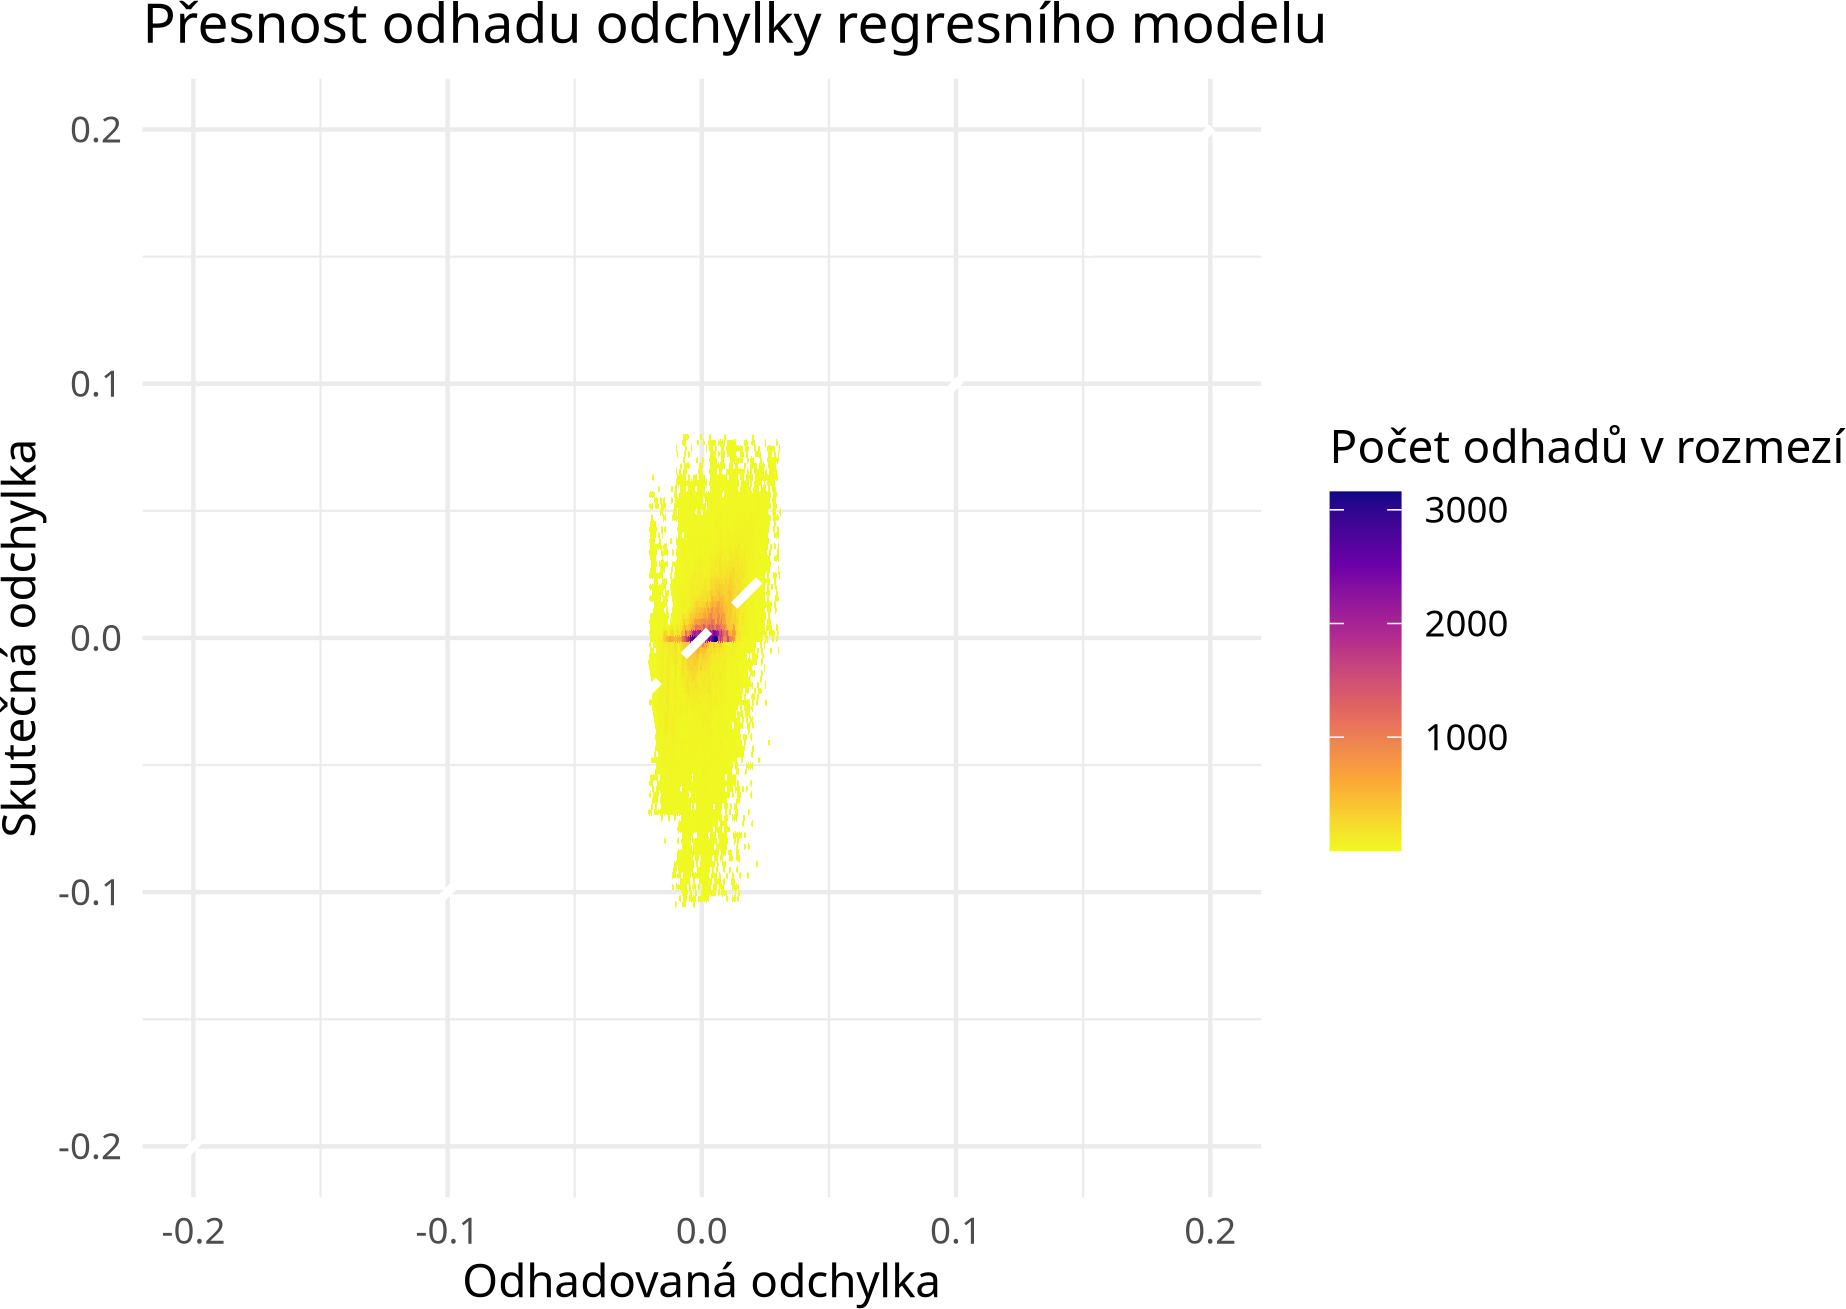
\includegraphics[keepaspectratio]{regression3_files/regression3_files/figure-latex/prediction_random_K-1.png}}

\begin{Shaded}
\begin{Highlighting}[]
\FunctionTok{anova}\NormalTok{(rmr\_relative)}
\end{Highlighting}
\end{Shaded}

\begin{verbatim}
## Type III Analysis of Variance Table with Satterthwaite's method
##            Sum Sq Mean Sq NumDF  DenDF   F value    Pr(>F)    
## moneyness 0.00248 0.00248     1 328370    8.9934  0.002710 ** 
## K         0.50811 0.50811     1 316310 1843.7988 < 2.2e-16 ***
## r         1.06873 1.06873     1 175814 3878.1228 < 2.2e-16 ***
## sigma     1.04381 1.04381     1 102445 3787.7217 < 2.2e-16 ***
## q         0.03160 0.03160     1   6502  114.6817 < 2.2e-16 ***
## T         2.31753 2.31753     1 329446 8409.6917 < 2.2e-16 ***
## am_eu     0.00384 0.00384     1     15   13.9484  0.001952 ** 
## call_put  0.70984 0.70984     1 329481 2575.8146 < 2.2e-16 ***
## model     0.00018 0.00009     2 329483    0.3229  0.724042    
## ---
## Signif. codes:  0 '***' 0.001 '**' 0.01 '*' 0.05 '.' 0.1 ' ' 1
\end{verbatim}

\begin{Shaded}
\begin{Highlighting}[]
\FunctionTok{ranef}\NormalTok{(rmr\_relative)}
\end{Highlighting}
\end{Shaded}

\begin{verbatim}
## $ticker
##         (Intercept)
## ^RUT   0.0195770209
## ^XDA  -0.0237926181
## ^XDB   0.0068772912
## ^XDE  -0.0053787670
## ^XDN   0.0027170730
## AAPL  -0.0115115258
## AMD    0.0112737067
## AMZN  -0.0032837207
## GOOGL  0.0036015244
## JNJ    0.0040604829
## KO    -0.0023659079
## META  -0.0021435765
## MSFT  -0.0029264114
## NFLX  -0.0022776730
## NVDA   0.0040244540
## PG    -0.0007873576
## TSLA   0.0023360061
## 
## $snapshot_month
##      (Intercept)
## 01 -0.0006723152
## 02  0.0007914657
## 03 -0.0006936764
## 05  0.0005745259
## 
## with conditional variances for "ticker" "snapshot_month"
\end{verbatim}

\subsection{LMER model - fixní efekty,
S}\label{lmer-model---fixnuxed-efekty-s}

Mnohem lepší \(R^2\), stále malé. Nevýznamný poměr \(S/K\) a styl
využití opce (a model).

\begin{Shaded}
\begin{Highlighting}[]
\NormalTok{subset\_args }\OtherTok{\textless{}{-}} \FunctionTok{c}\NormalTok{(}
  \StringTok{"S"}\NormalTok{,}
  \StringTok{"moneyness"}\NormalTok{,}
  \CommentTok{\#"K",}
  \StringTok{"r"}\NormalTok{,}
  \StringTok{"sigma"}\NormalTok{,}
  \StringTok{"q"}\NormalTok{,}
  \StringTok{"T"}\NormalTok{,}
  \StringTok{"am\_eu"}\NormalTok{,}
  \StringTok{"call\_put"}\NormalTok{,}
  \StringTok{"model"}\NormalTok{,}
  \StringTok{"ticker"}\NormalTok{,}
  \StringTok{"snapshot\_month"}
\NormalTok{)}
\NormalTok{interactions }\OtherTok{\textless{}{-}} \FunctionTok{c}\NormalTok{()}

\NormalTok{rhs }\OtherTok{\textless{}{-}} \FunctionTok{paste}\NormalTok{(}\FunctionTok{c}\NormalTok{(subset\_args, interactions), }\AttributeTok{collapse =} \StringTok{" + "}\NormalTok{)}
\NormalTok{formula }\OtherTok{\textless{}{-}} \FunctionTok{as.formula}\NormalTok{(}\FunctionTok{paste}\NormalTok{(}\StringTok{"pricing\_error \textasciitilde{} "}\NormalTok{, rhs))}

\NormalTok{rmr\_relative }\OtherTok{\textless{}{-}} \FunctionTok{lm}\NormalTok{(formula, }\AttributeTok{data =}\NormalTok{ train\_data\_rel)}
\end{Highlighting}
\end{Shaded}

\begin{Shaded}
\begin{Highlighting}[]
\FunctionTok{summary}\NormalTok{(rmr\_relative)}
\end{Highlighting}
\end{Shaded}

\begin{verbatim}
## 
## Call:
## lm(formula = formula, data = train_data_rel)
## 
## Residuals:
##       Min        1Q    Median        3Q       Max 
## -0.116219 -0.005524  0.000993  0.007449  0.083786 
## 
## Coefficients: (1 not defined because of singularities)
##                    Estimate Std. Error t value Pr(>|t|)    
## (Intercept)      -3.375e-02  1.290e-03 -26.161  < 2e-16 ***
## S                 7.251e-06  5.999e-07  12.087  < 2e-16 ***
## moneyness         8.024e-04  2.873e-05  27.927  < 2e-16 ***
## r                 1.796e+00  2.863e-02  62.746  < 2e-16 ***
## sigma            -8.284e-02  1.266e-03 -65.440  < 2e-16 ***
## q                -4.644e-01  4.977e-02  -9.330  < 2e-16 ***
## T                 3.702e-03  4.180e-05  88.559  < 2e-16 ***
## am_eueuropean    -3.502e-02  1.506e-03 -23.261  < 2e-16 ***
## call_putputs     -2.514e-03  5.920e-05 -42.465  < 2e-16 ***
## modeluser_crr    -1.585e-05  7.099e-05  -0.223 0.823332    
## modeluser_mc     -5.610e-05  7.103e-05  -0.790 0.429661    
## ticker^XDA       -8.834e-03  2.439e-03  -3.621 0.000293 ***
## ticker^XDB        2.129e-02  2.179e-03   9.772  < 2e-16 ***
## ticker^XDE        9.336e-03  1.876e-03   4.977 6.45e-07 ***
## ticker^XDN        1.870e-02  2.072e-03   9.027  < 2e-16 ***
## tickerAAPL       -1.345e-02  4.250e-04 -31.645  < 2e-16 ***
## tickerAMD         1.119e-02  1.755e-04  63.794  < 2e-16 ***
## tickerAMZN       -4.030e-03  3.235e-04 -12.460  < 2e-16 ***
## tickerGOOGL       9.788e-04  4.096e-04   2.390 0.016866 *  
## tickerJNJ         5.074e-04  1.746e-03   0.291 0.771325    
## tickerKO         -3.745e-03  1.591e-03  -2.354 0.018573 *  
## tickerMETA       -8.830e-03  3.468e-04 -25.460  < 2e-16 ***
## tickerMSFT       -7.426e-03  5.742e-04 -12.933  < 2e-16 ***
## tickerNFLX       -1.248e-03  3.414e-04  -3.654 0.000258 ***
## tickerNVDA        4.047e-03  2.465e-04  16.419  < 2e-16 ***
## tickerPG         -2.826e-03  1.443e-03  -1.958 0.050172 .  
## tickerTSLA               NA         NA      NA       NA    
## snapshot_month02  1.640e-03  8.513e-05  19.261  < 2e-16 ***
## snapshot_month03  5.114e-04  9.636e-05   5.307 1.12e-07 ***
## snapshot_month05  2.672e-04  1.154e-04   2.317 0.020528 *  
## ---
## Signif. codes:  0 '***' 0.001 '**' 0.01 '*' 0.05 '.' 0.1 ' ' 1
## 
## Residual standard error: 0.01664 on 329483 degrees of freedom
## Multiple R-squared:  0.1686, Adjusted R-squared:  0.1685 
## F-statistic:  2386 on 28 and 329483 DF,  p-value: < 2.2e-16
\end{verbatim}

\begin{Shaded}
\begin{Highlighting}[]
\FunctionTok{r2}\NormalTok{(rmr\_relative)}
\end{Highlighting}
\end{Shaded}

\begin{verbatim}
## # R2 for Linear Regression
##        R2: 0.169
##   adj. R2: 0.168
\end{verbatim}

\begin{verbatim}
## Model matrix is rank deficient. Parameters `tickerTSLA` were not
##   estimable.
\end{verbatim}

\pandocbounded{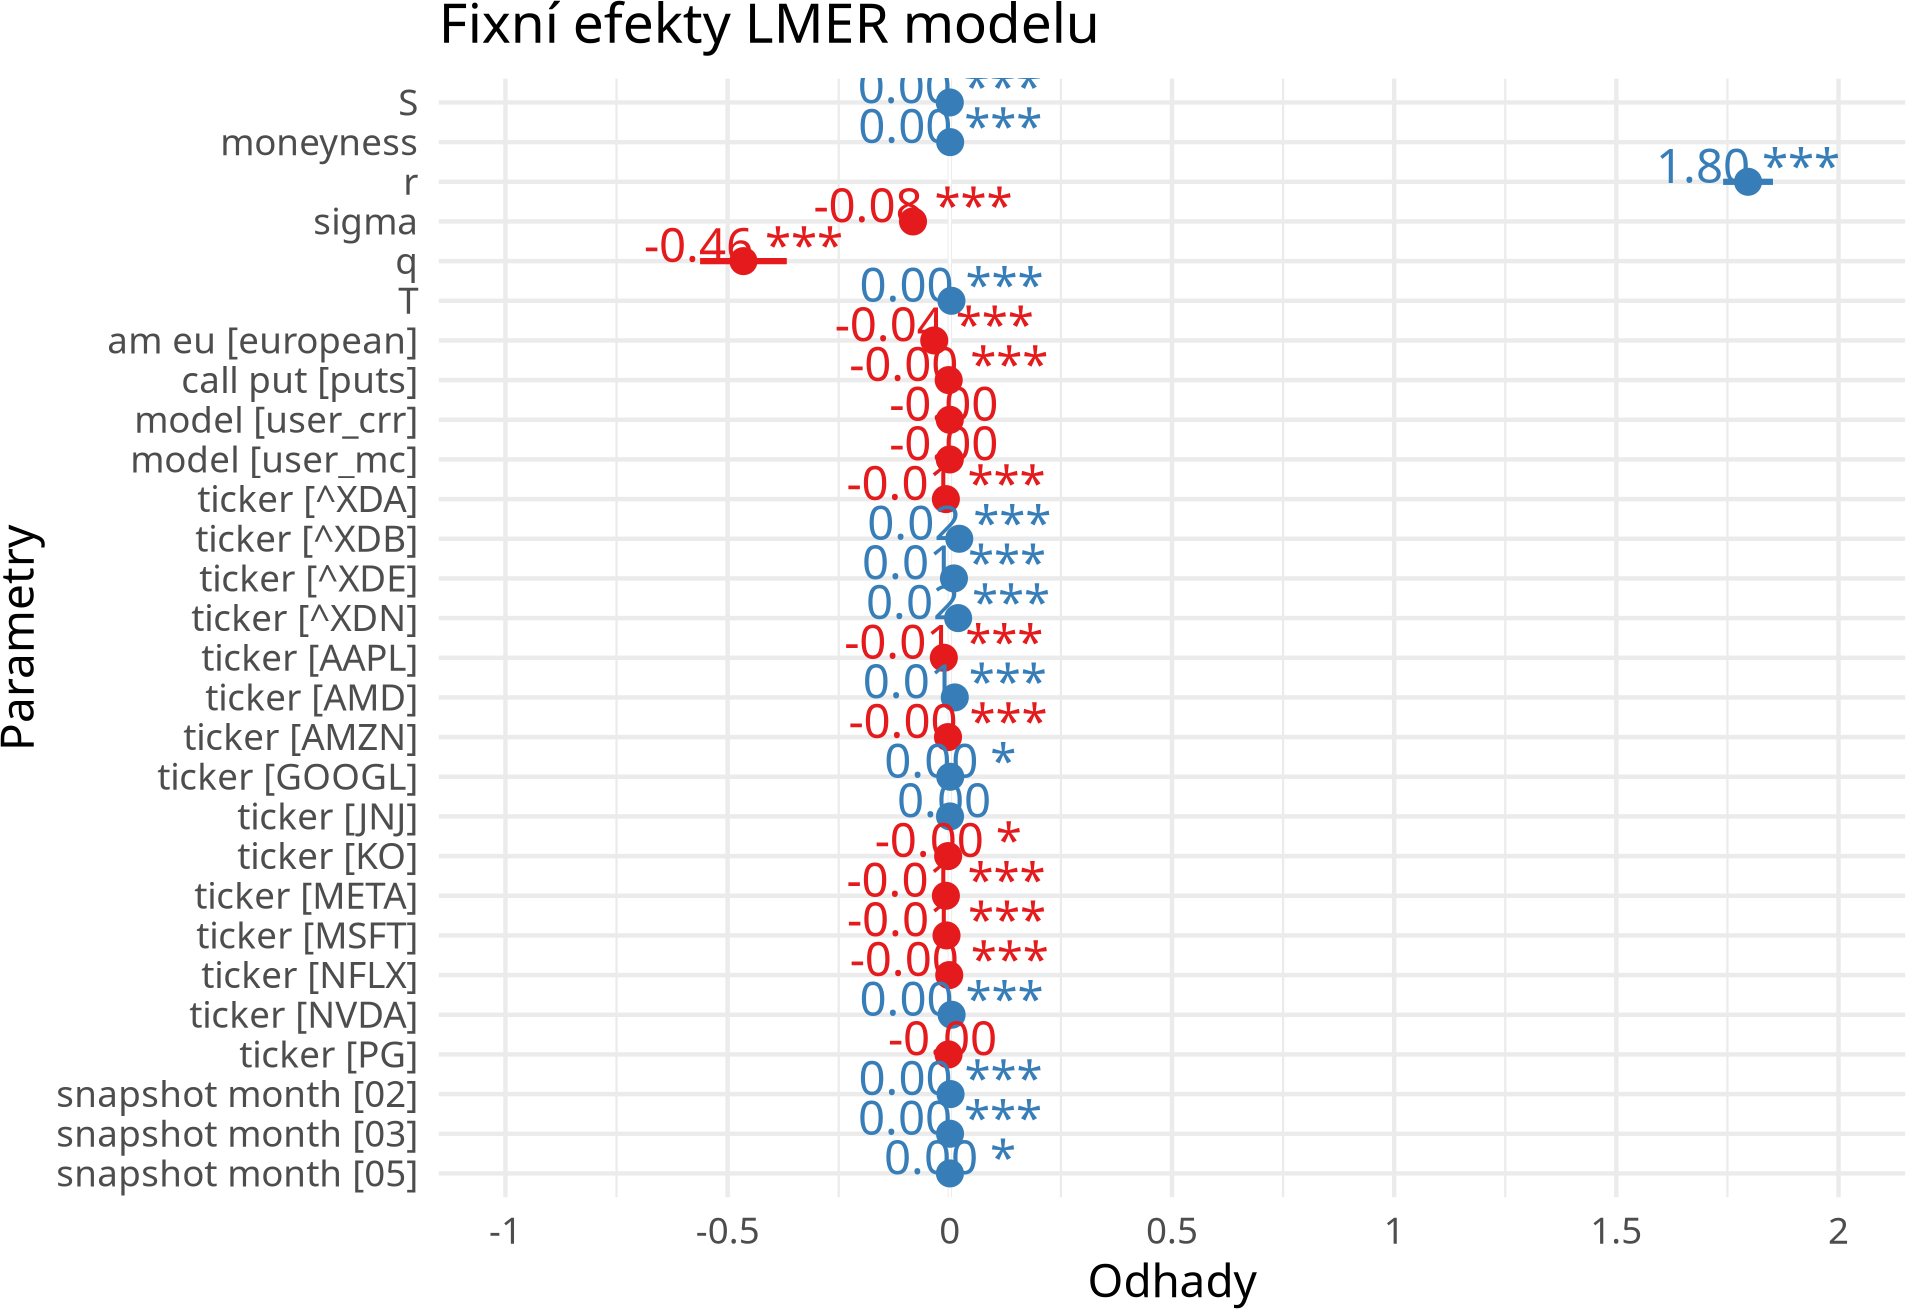
\includegraphics[keepaspectratio]{regression3_files/regression3_files/figure-latex/unnamed-chunk-13-1.png}}

\pandocbounded{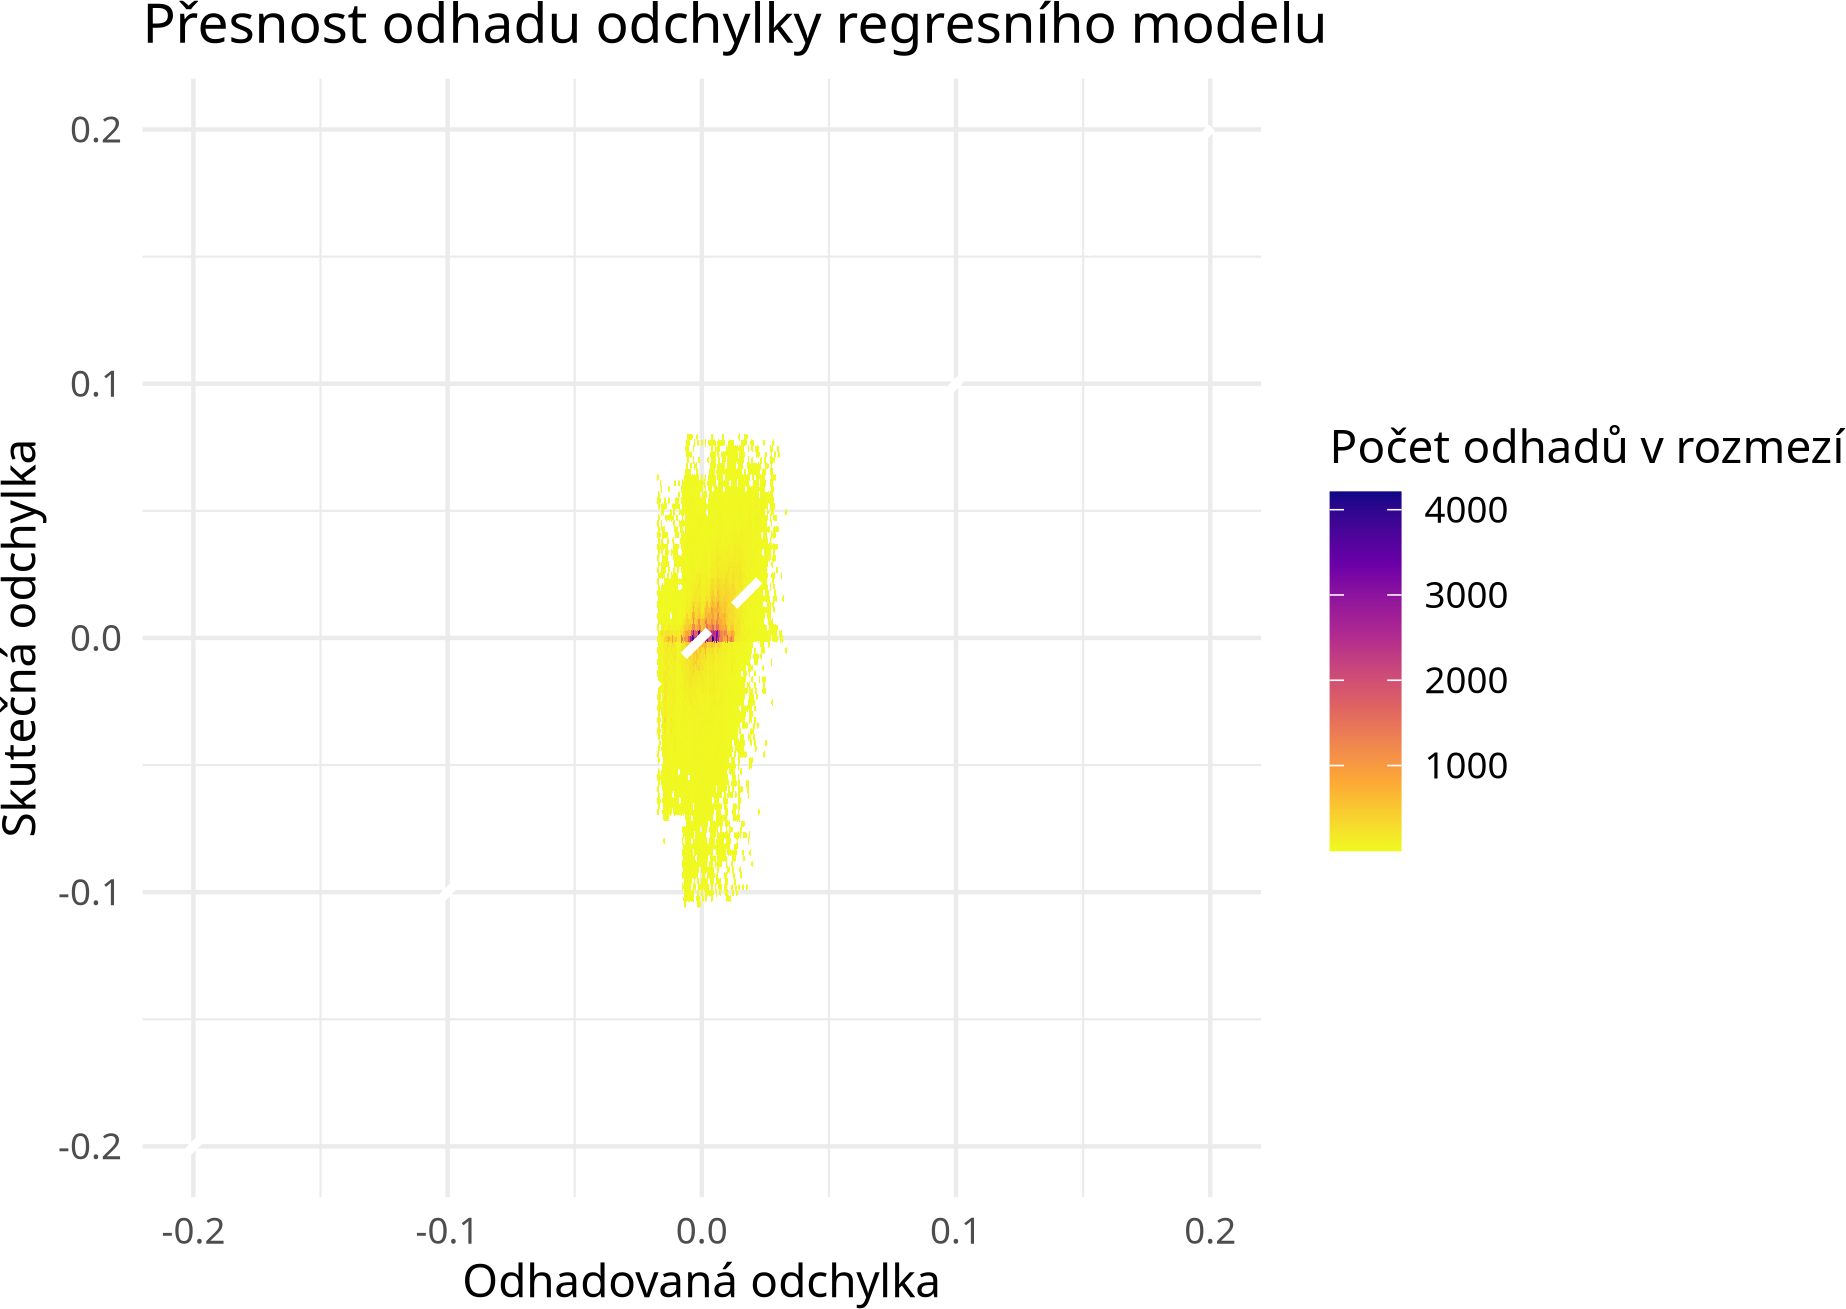
\includegraphics[keepaspectratio]{regression3_files/regression3_files/figure-latex/prediction_fixed_S-1.png}}

\begin{Shaded}
\begin{Highlighting}[]
\FunctionTok{anova}\NormalTok{(rmr\_relative)}
\end{Highlighting}
\end{Shaded}

\begin{verbatim}
## Analysis of Variance Table
## 
## Response: pricing_error
##                    Df Sum Sq Mean Sq    F value Pr(>F)    
## S                   1  0.423  0.4234  1528.5356 <2e-16 ***
## moneyness           1  0.093  0.0932   336.5894 <2e-16 ***
## r                   1  1.893  1.8934  6835.1815 <2e-16 ***
## sigma               1  6.859  6.8586 24760.0831 <2e-16 ***
## q                   1  1.096  1.0960  3956.4833 <2e-16 ***
## T                   1  2.149  2.1494  7759.4271 <2e-16 ***
## am_eu               1  0.069  0.0693   250.1558 <2e-16 ***
## call_put            1  0.520  0.5199  1876.9180 <2e-16 ***
## model               2  0.000  0.0001     0.3163 0.7288    
## ticker             15  5.295  0.3530  1274.2803 <2e-16 ***
## snapshot_month      3  0.106  0.0353   127.3656 <2e-16 ***
## Residuals      329483 91.267  0.0003                      
## ---
## Signif. codes:  0 '***' 0.001 '**' 0.01 '*' 0.05 '.' 0.1 ' ' 1
\end{verbatim}

\begin{Shaded}
\begin{Highlighting}[]
\FunctionTok{ranef}\NormalTok{(rmr\_relative)}
\end{Highlighting}
\end{Shaded}

\subsection{LMER model - náhodné efekty,
S}\label{lmer-model---nuxe1hodnuxe9-efekty-s}

Mnohem lepší \(R^2\), stále malé. Nevýznamný poměr \(S/K\) a styl
využití opce (a model).

\begin{Shaded}
\begin{Highlighting}[]
\NormalTok{subset\_args }\OtherTok{\textless{}{-}} \FunctionTok{c}\NormalTok{(}
  \StringTok{"S"}\NormalTok{,}
  \StringTok{"moneyness"}\NormalTok{,}
  \CommentTok{\#"K",}
  \StringTok{"r"}\NormalTok{,}
  \StringTok{"sigma"}\NormalTok{,}
  \StringTok{"q"}\NormalTok{,}
  \StringTok{"T"}\NormalTok{,}
  \StringTok{"am\_eu"}\NormalTok{,}
  \StringTok{"call\_put"}\NormalTok{,}
  \StringTok{"model"}
  \CommentTok{\#"ticker"}
\NormalTok{)}
\NormalTok{interactions }\OtherTok{\textless{}{-}} \FunctionTok{c}\NormalTok{(}
  \StringTok{"(1 | ticker)"}\NormalTok{,}
  \StringTok{"(1 | snapshot\_month)"}
\NormalTok{)}

\NormalTok{rhs }\OtherTok{\textless{}{-}} \FunctionTok{paste}\NormalTok{(}\FunctionTok{c}\NormalTok{(subset\_args, interactions), }\AttributeTok{collapse =} \StringTok{" + "}\NormalTok{)}
\NormalTok{formula }\OtherTok{\textless{}{-}} \FunctionTok{as.formula}\NormalTok{(}\FunctionTok{paste}\NormalTok{(}\StringTok{"pricing\_error \textasciitilde{} "}\NormalTok{, rhs))}

\NormalTok{rmr\_relative }\OtherTok{\textless{}{-}} \FunctionTok{lmer}\NormalTok{(formula, }\AttributeTok{data =}\NormalTok{ train\_data\_rel)}
\end{Highlighting}
\end{Shaded}

\begin{verbatim}
## Warning: Some predictor variables are on very different scales: consider rescaling. 
## You may also use (g)lmerControl(autoscale = TRUE) to improve numerical stability.
## Warning: Some predictor variables are on very different scales: consider rescaling. 
## You may also use (g)lmerControl(autoscale = TRUE) to improve numerical stability.
\end{verbatim}

\begin{Shaded}
\begin{Highlighting}[]
\FunctionTok{summary}\NormalTok{(rmr\_relative)}
\end{Highlighting}
\end{Shaded}

\begin{verbatim}
## Linear mixed model fit by REML. t-tests use Satterthwaite's method [
## lmerModLmerTest]
## Formula: formula
##    Data: train_data_rel
## 
## REML criterion at convergence: -1763792
## 
## Scaled residuals: 
##     Min      1Q  Median      3Q     Max 
## -6.9820 -0.3319  0.0596  0.4473  5.0350 
## 
## Random effects:
##  Groups         Name        Variance  Std.Dev. 
##  ticker         (Intercept) 6.971e-05 0.0083493
##  snapshot_month (Intercept) 5.123e-07 0.0007158
##  Residual                   2.770e-04 0.0166434
## Number of obs: 329512, groups:  ticker, 17; snapshot_month, 4
## 
## Fixed effects:
##                 Estimate Std. Error         df t value Pr(>|t|)    
## (Intercept)   -3.512e-02  2.734e-03  2.350e+01 -12.847 4.09e-12 ***
## S              7.104e-06  5.902e-07  1.612e+04  12.036  < 2e-16 ***
## moneyness      8.024e-04  2.873e-05  3.295e+05  27.927  < 2e-16 ***
## r              1.794e+00  2.858e-02  1.374e+05  62.792  < 2e-16 ***
## sigma         -8.264e-02  1.259e-03  5.332e+04 -65.645  < 2e-16 ***
## q             -4.684e-01  4.821e-02  3.707e+03  -9.716  < 2e-16 ***
## T              3.701e-03  4.180e-05  3.294e+05  88.551  < 2e-16 ***
## am_eueuropean -2.478e-02  4.523e-03  1.531e+01  -5.479 5.90e-05 ***
## call_putputs  -2.513e-03  5.920e-05  3.295e+05 -42.457  < 2e-16 ***
## modeluser_crr -1.580e-05  7.099e-05  3.295e+05  -0.223    0.824    
## modeluser_mc  -5.606e-05  7.103e-05  3.295e+05  -0.789    0.430    
## ---
## Signif. codes:  0 '***' 0.001 '**' 0.01 '*' 0.05 '.' 0.1 ' ' 1
## 
## Correlation of Fixed Effects:
##             (Intr) S      mnynss r      sigma  q      T      am_rpn cll_pt
## S           -0.054                                                        
## moneyness   -0.014 -0.024                                                 
## r           -0.387  0.029  0.017                                          
## sigma       -0.149 -0.179 -0.023 -0.003                                   
## q           -0.168  0.071  0.008 -0.022  0.038                            
## T           -0.069  0.003 -0.074  0.158 -0.013  0.001                     
## am_eueuropn -0.494 -0.050  0.002 -0.004  0.075  0.100  0.002              
## call_putpts -0.003  0.007 -0.169 -0.012  0.000 -0.002 -0.003  0.000       
## modelsr_crr -0.013  0.000  0.000 -0.001  0.000 -0.001  0.000  0.000  0.000
## modelusr_mc -0.013  0.001 -0.001 -0.001  0.000  0.000  0.000  0.000  0.000
##             mdlsr_c
## S                  
## moneyness          
## r                  
## sigma              
## q                  
## T                  
## am_eueuropn        
## call_putpts        
## modelsr_crr        
## modelusr_mc  0.500 
## fit warnings:
## Some predictor variables are on very different scales: consider rescaling. 
## You may also use (g)lmerControl(autoscale = TRUE) to improve numerical stability.
\end{verbatim}

\begin{Shaded}
\begin{Highlighting}[]
\FunctionTok{r2}\NormalTok{(rmr\_relative)}
\end{Highlighting}
\end{Shaded}

\begin{verbatim}
## Warning: Can't compute random effect variances. Some variance components equal
##   zero. Your model may suffer from singularity (see `?lme4::isSingular`
##   and `?performance::check_singularity`).
##   Decrease the `tolerance` level to force the calculation of random effect
##   variances, or impose priors on your random effects parameters (using
##   packages like `brms` or `glmmTMB`).
\end{verbatim}

\begin{verbatim}
## Random effect variances not available. Returned R2 does not account for random effects.
\end{verbatim}

\begin{verbatim}
## # R2 for Mixed Models
## 
##   Conditional R2: NA
##      Marginal R2: 0.246
\end{verbatim}

\pandocbounded{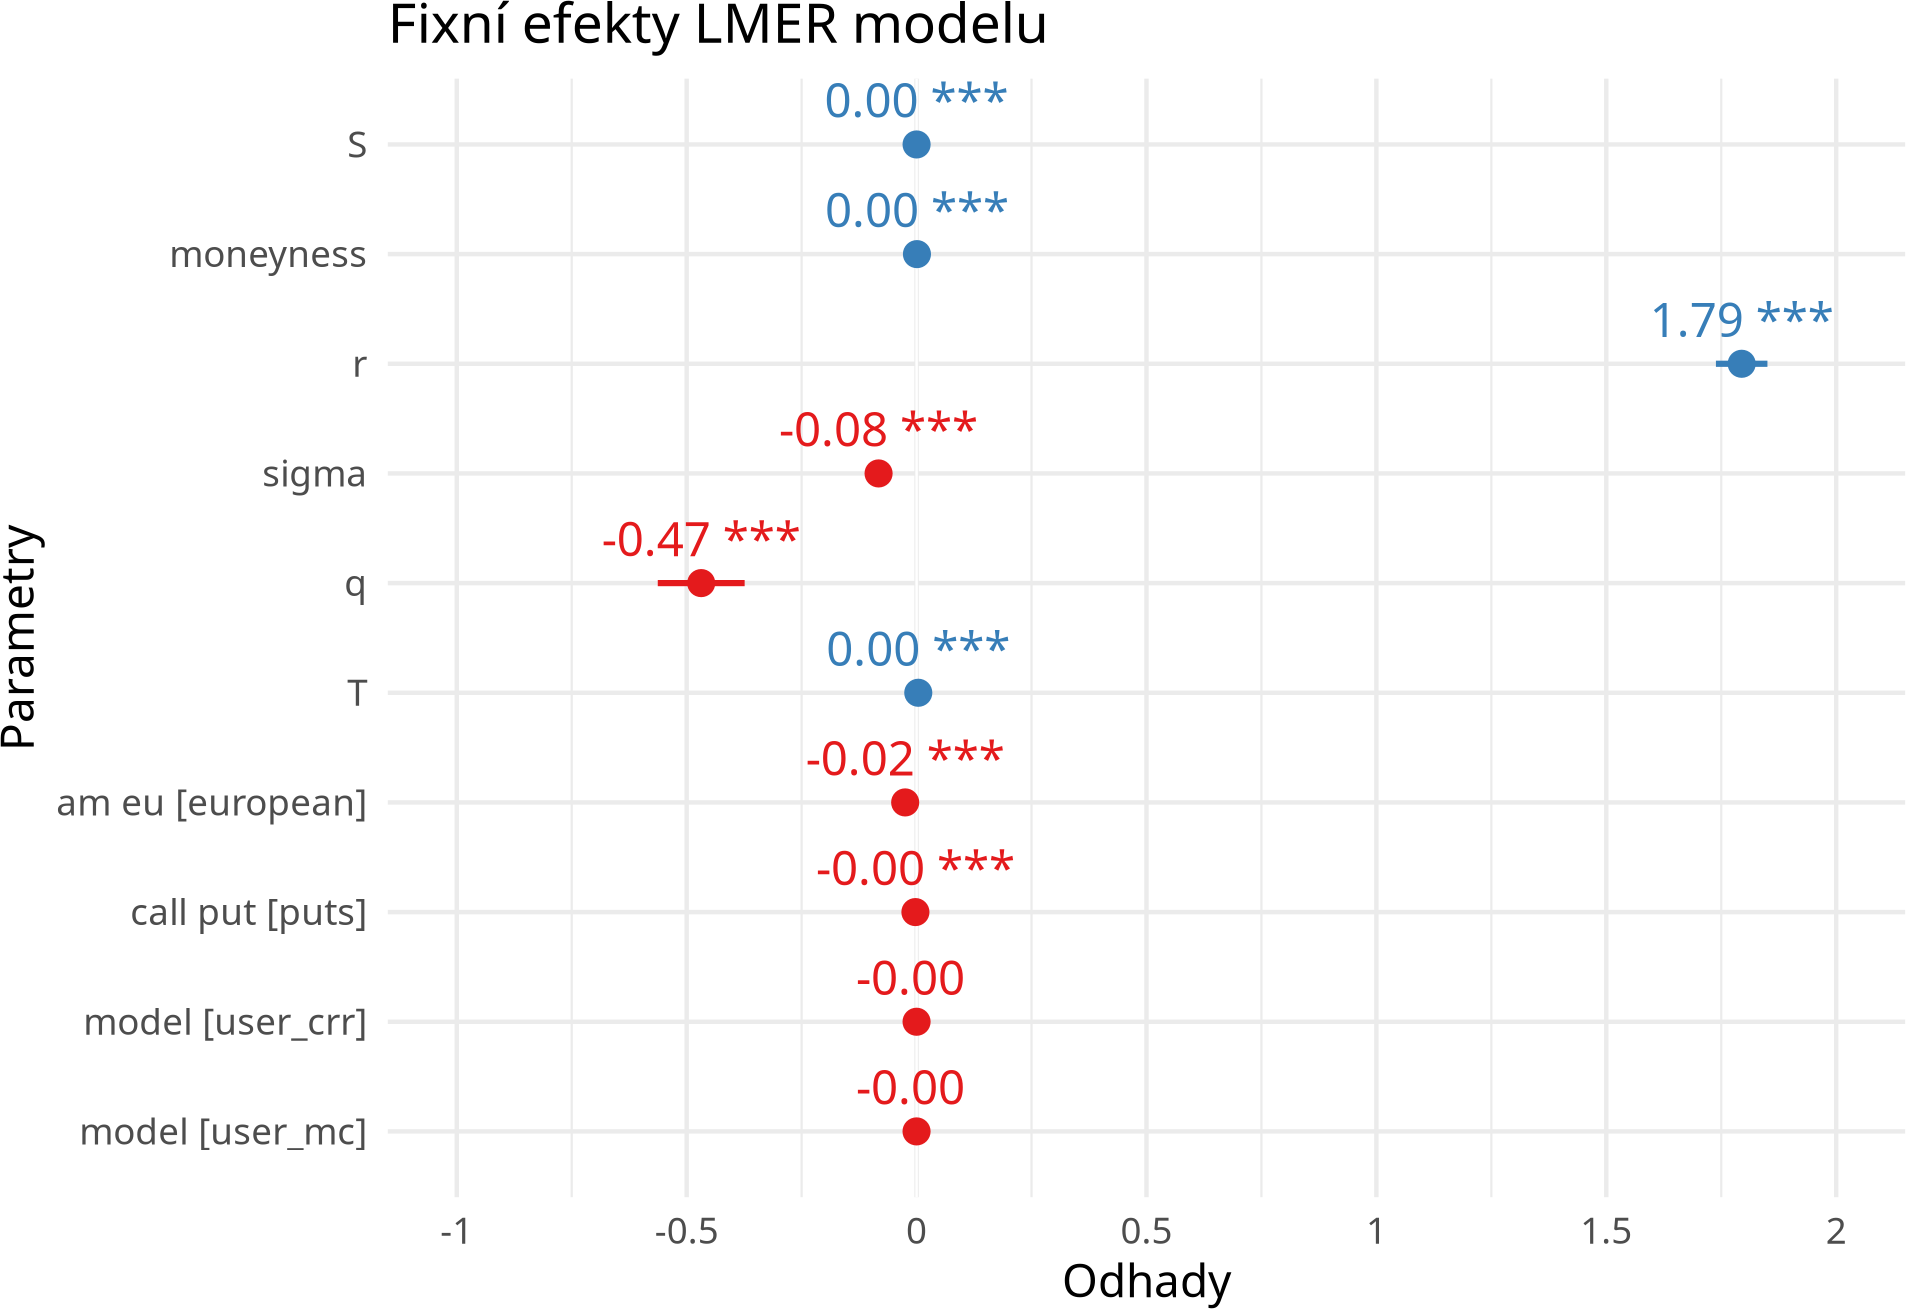
\includegraphics[keepaspectratio]{regression3_files/regression3_files/figure-latex/unnamed-chunk-18-1.png}}

\pandocbounded{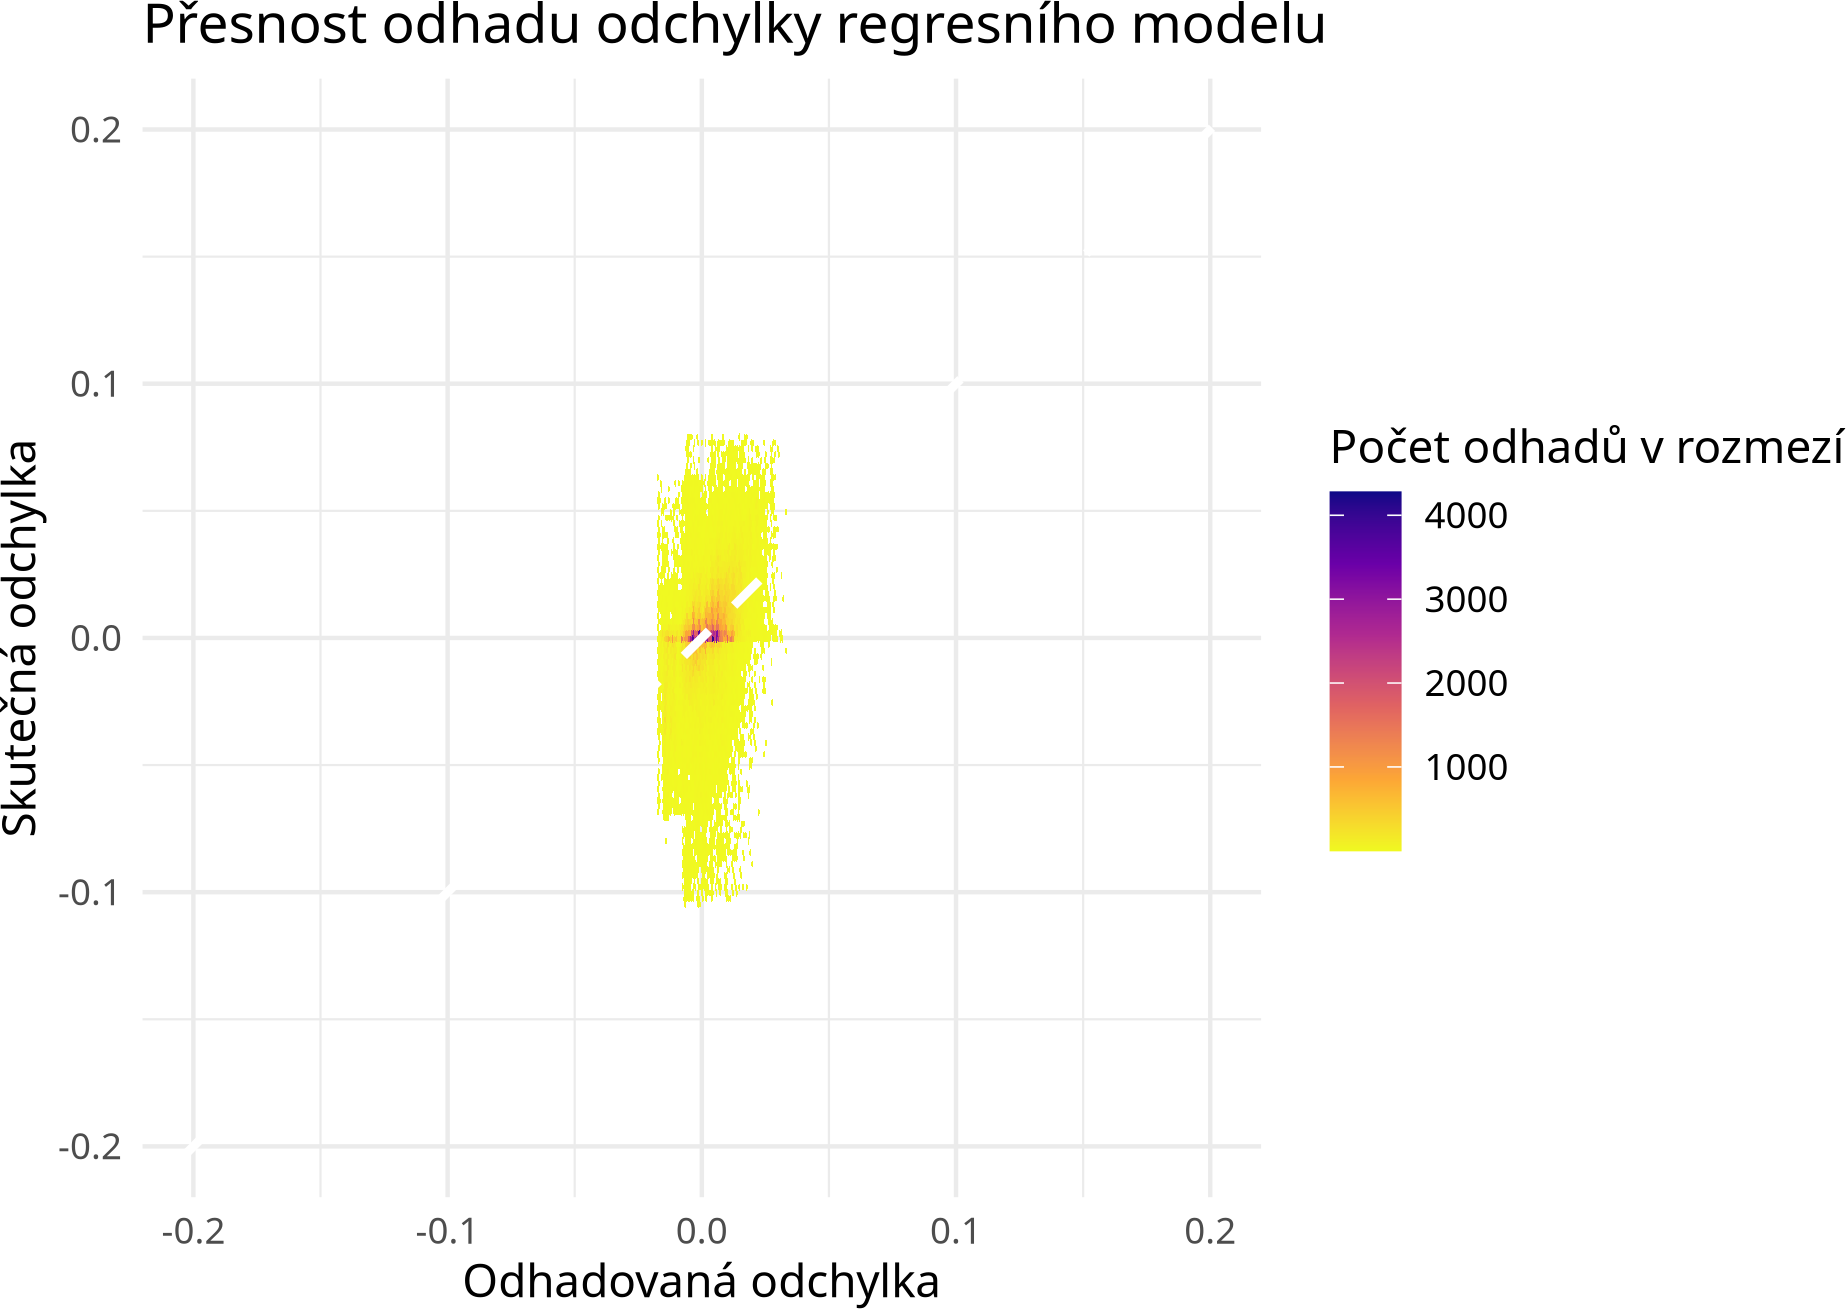
\includegraphics[keepaspectratio]{regression3_files/regression3_files/figure-latex/prediction_random_S-1.png}}

\begin{Shaded}
\begin{Highlighting}[]
\FunctionTok{anova}\NormalTok{(rmr\_relative)}
\end{Highlighting}
\end{Shaded}

\begin{verbatim}
## Type III Analysis of Variance Table with Satterthwaite's method
##            Sum Sq Mean Sq NumDF  DenDF  F value    Pr(>F)    
## S         0.04013 0.04013     1  16123  144.867 < 2.2e-16 ***
## moneyness 0.21604 0.21604     1 329498  779.910 < 2.2e-16 ***
## r         1.09217 1.09217     1 137377 3942.815 < 2.2e-16 ***
## sigma     1.19369 1.19369     1  53316 4309.307 < 2.2e-16 ***
## q         0.02615 0.02615     1   3707   94.409 < 2.2e-16 ***
## T         2.17204 2.17204     1 329397 7841.243 < 2.2e-16 ***
## am_eu     0.00832 0.00832     1     15   30.019 5.903e-05 ***
## call_put  0.49933 0.49933     1 329497 1802.610 < 2.2e-16 ***
## model     0.00018 0.00009     2 329483    0.331    0.7182    
## ---
## Signif. codes:  0 '***' 0.001 '**' 0.01 '*' 0.05 '.' 0.1 ' ' 1
\end{verbatim}

\begin{Shaded}
\begin{Highlighting}[]
\FunctionTok{ranef}\NormalTok{(rmr\_relative)}
\end{Highlighting}
\end{Shaded}

\begin{verbatim}
## $ticker
##         (Intercept)
## ^RUT  -0.0078312635
## ^XDA  -0.0162007009
## ^XDB   0.0126606687
## ^XDE   0.0011352850
## ^XDN   0.0102360106
## AAPL  -0.0113890886
## AMD    0.0131711571
## AMZN  -0.0020050643
## GOOGL  0.0030418080
## JNJ    0.0026957701
## KO    -0.0015875867
## META  -0.0067428299
## MSFT  -0.0053244298
## NFLX   0.0007565412
## NVDA   0.0060507186
## PG    -0.0006749605
## TSLA   0.0020079642
## 
## $snapshot_month
##      (Intercept)
## 01 -0.0006025341
## 02  0.0010221480
## 03 -0.0001004766
## 05 -0.0003191372
## 
## with conditional variances for "ticker" "snapshot_month"
\end{verbatim}

\end{document}
